\section{Design af user interfacet}
I dette afsnit vil vi beskrive det generelle design af brugergrænsefladen og de beslutninger der ligger bag.

\subsection{Generelle mål med user interfacet}
Da den første UI skulle designes havde vi fokus på fire ting:
\begin{itemize}
\item Strømlignet interface
\item Nem navigering
\item Intuitivt design
\item Ease of use
\end{itemize}
\paragraph{Strømlignet interface}
Igennem hele designfasen havde vi fokus på, at user interfacet var strømlignet det vil sige, at vi prøvede at designe skærmbillederne således, at de alle havde den samme grund strukturt og derfor minde mere om hinaden.
\paragraph{Nem navigering}
Vi ville også gerne have at det var nemt at navigere rundt i systemtet, så vi stillede altid mod, at man ville kunne skifte til alle sidder med 1-2 klik fra ens skærmbilled.
\paragraph{Intuitivt design}
En vigtig faktor for os var også, at systemet var intuitivt at bruge, vores udgangspunkt var derfor at prøve at lave et system der mindede om noget man var vant  til at se fra andre booking systemer.
\paragraph{Ease of use}\footnote{User Interface Design, side 9}
Som overordnet tema fokuserede vi på, at systemet skylle have høj Ease of use, hvilket blandet andet indebære at det skal være hurtigt og nemt at bruge dageligt, det var derfor vigtigt at det blev lavet til en hurtig og nem tilgængelig platform. Derfor valgt vi at kode det som en hjemmeside.

\subsection{Booking metoden}
Som nævnt ville vi gerne prøve at efterligne eksisterende booking systemer, specielt blev vi meget inspireret af biografbooking dette skyldtes, at det er et meget intuitivt systmet hvilket vi også gerne vil opnå.\\ Konceptet med, at visuelt vælge hvad man vil have og deres simple farvekodning var noget der passede godt ind i vores koncept med ease of use og intuitivt design.
\begin{figure}[h!]
  \caption{screenshot af kino.dk's booking interface.}
  \centering
    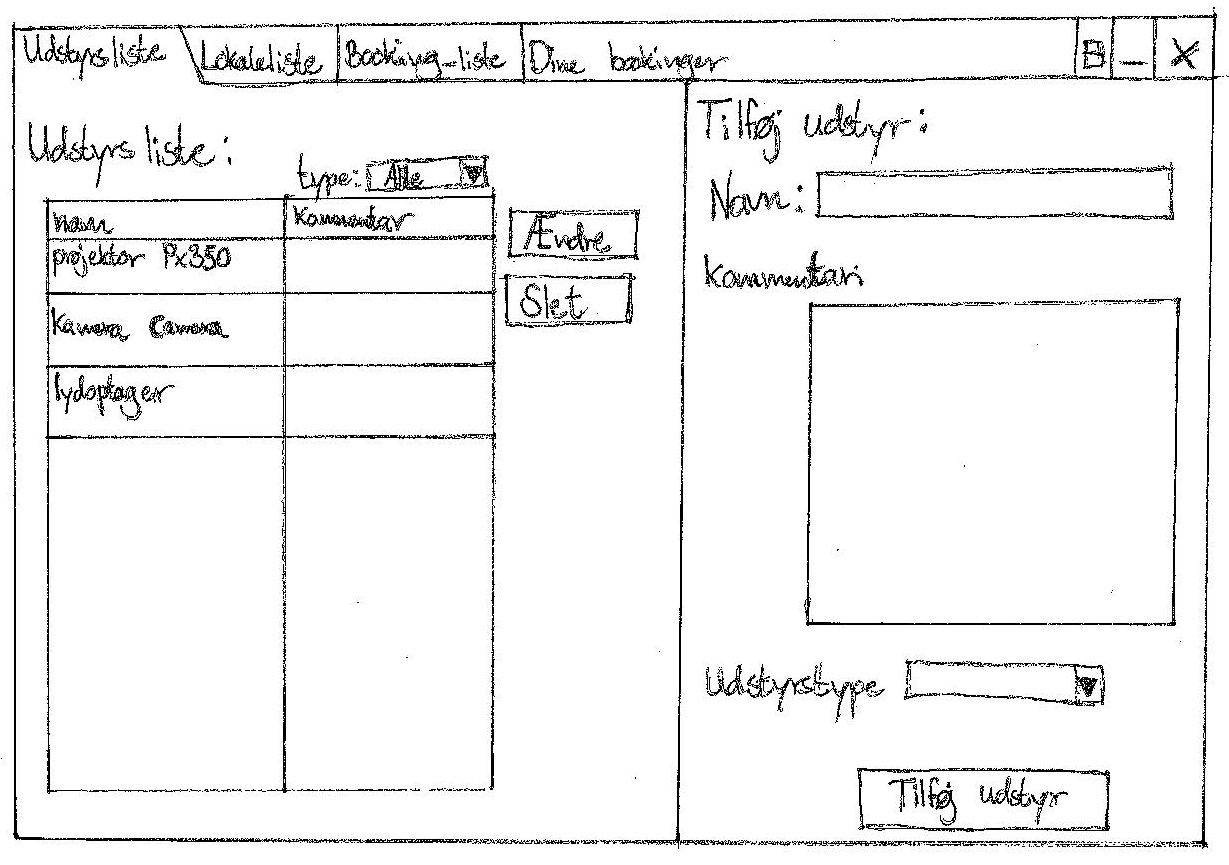
\includegraphics[width=0.5\textwidth]{Appendix/GUI-Prototype/PaperMockup/UdstyrsListe}
\end{figure}


Vi valgte at prøve at efterligne det ved at lave et gitter hvor man kunne klikke i felterne for at booke et lokale i det tilsvarende tidsrum, det viste sig dog af vores første usability test\footnote{resultat af usability test1}, at den løsning ikke var helt brugervenlig nok vi valgte derfor at tilføje checkboxses til alle felterne for at gøre det mere tydeligt, at det var det der skulle markes for at booke et lokale i et givent tidsrum.
\begin{figure}[h!]
\label{GitterBook}
  \caption{Den endelige udgave af gitter skærmbilleder til booking.}
  \centering
    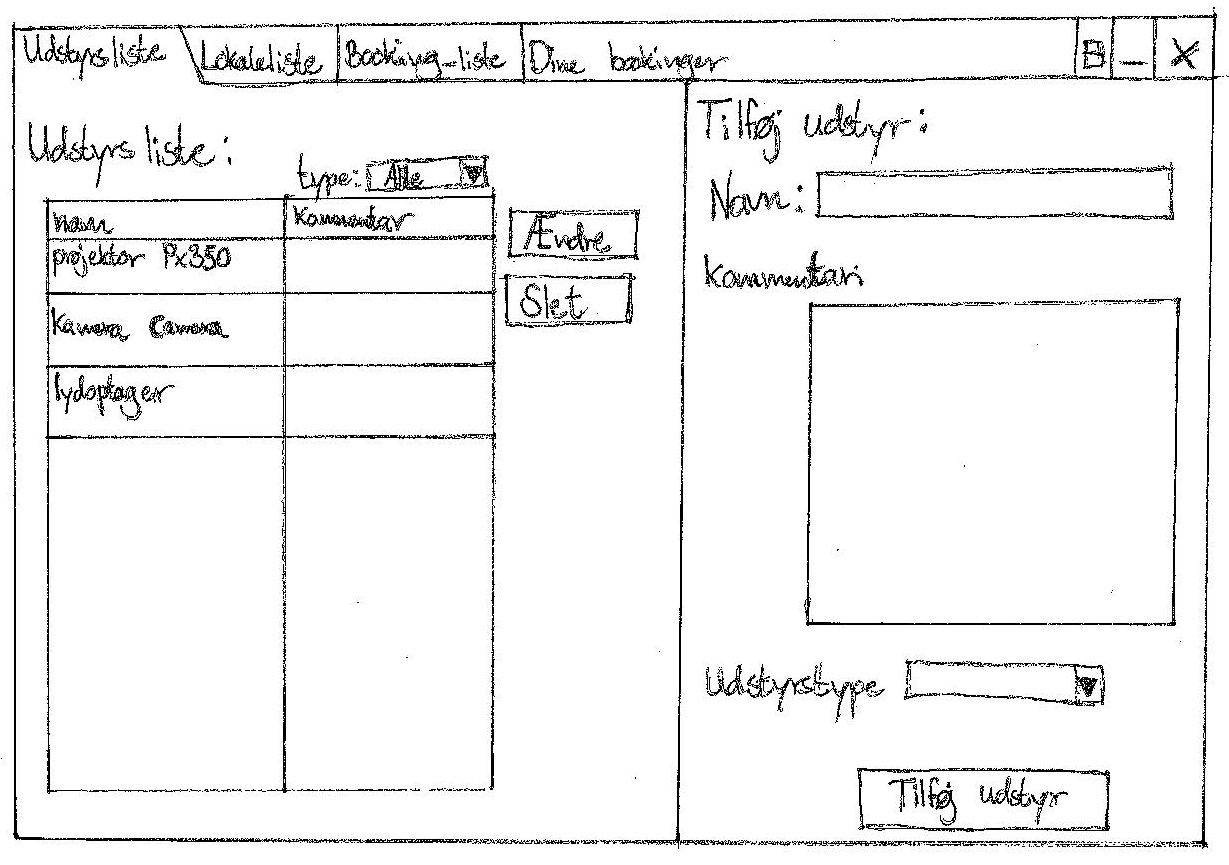
\includegraphics[width=0.5\textwidth]{Appendix/GUI-Prototype/PaperMockup/UdstyrsListe}
\end{figure}
\\Da vi gerne vil opnå en brugergrænseflade som var strømlignet og nem at bruge, brugte vi også gitter løsningen til alt andet der relaterede til en booking i systemt såsom tilføjelse af  udstyr og forplejning. Til resten af skærm billederne har vi holdt os til simple billeder der fokusere på kun at præsentere den nødvendige datae og knapper.

\subsection{UI'ens udvikling og udseende}
Til UI'ens generelle udseende gik vi efter, at der skulle være meget få forskellige skærmbilleder således at der måske var 10-15 skærmbilleder, men for brugen skulle vedkommende kun lære at navigere igennem et par stykker for at kende systemet.
Generelt kan man opdele skærmbillederne i to typer, den første type er alle dem som indholder booking gitterer.
Figur \ref{Gitterbook}er et screenshot af vores endelig design af et af gitter skærmbillederne.
\begin{figure}[h!]
\label{PapirGitterBook}
  \caption{første udgave af gitter skærmbilleder til booking.}
  \centering
    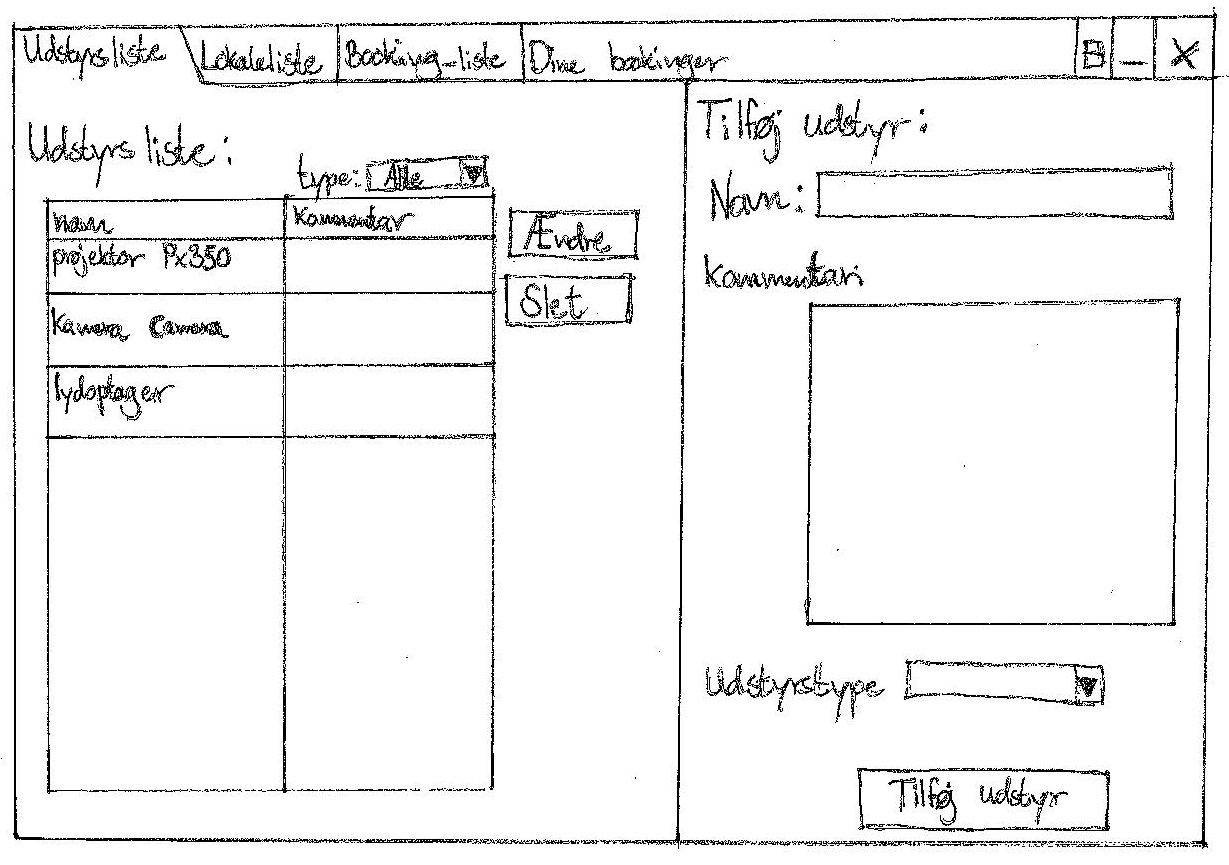
\includegraphics[width=0.5\textwidth]{Appendix/GUI-Prototype/PaperMockup/UdstyrsListe}
\end{figure}

Figur \ref{PapirGitterBook} viser det skærmbilled der blev brugt til at lave den første runde af usability test på en simpel papir mockup, som man kan se minder den i sin form om det endelig version men der nogle små forskelle, det vigtigste er tilføjelsen af checkboxses. Disse blev tilføjet efter første runde af usabilitytests da feedbacken var, at der manglede noget man kunne klikke på i gitteret, derudover gjorde vi også knapperne mere merkante og gav dem et fælles layout så det var meget tydligt hvad der var klikbare knapper.

Den anden type af skærmbilleder er primært til editering i de forskellige tabeller der er i systemet det kunne eksempelvis være oversigten over lokaler hvor man er i stand til at ændre, slette og tilføje lokaler.
I den første udgave i papir mockupen var disse meget simple og manglede noget information om hvad der blev vist.
\begin{figure}[h!]
  \caption{første udgave af skærmbilled over en liste af bookinger der skal godkendes af receptionisten.}
  \centering
    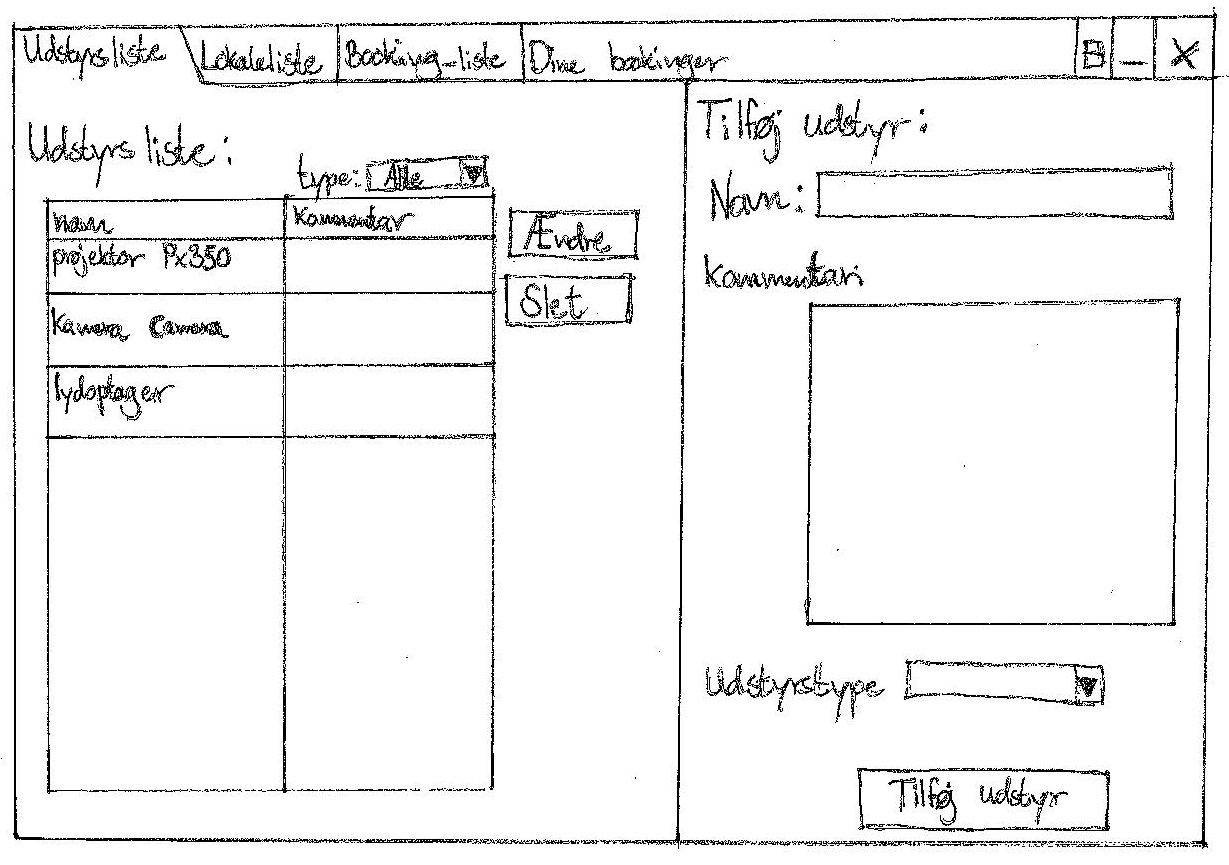
\includegraphics[width=0.5\textwidth]{Appendix/GUI-Prototype/PaperMockup/UdstyrsListe}
\end{figure} 
I forhold til det generelle design af skærmbillederne prøvede vi at gøre dem simple og at overholde gestalt lovene\footnote{User Interface Design, side 68} specifikt Law of proximity. Således at det virker som om knapper intuitivt tilhører til den liste, som de interegere med.




